\documentclass{mythesis}
\usepackage{mythesis}

%% You can set the line spacing this way
%\setallspacing{double}
%% or a section at a time like this
%\setfrontmatterspacing{double}

%% PDF metadata
\makeatletter
\@ifpackageloaded{hyperref}{%
\hypersetup{%
pdftitle = {Collaborative Video streaming for Mobile Devices},
pdfsubject = {Mobilnetze, dienstintegrierte Netze und Echtzeitkommunikation},
pdfkeywords = {Video, Streaming, Mobile},
pdfauthor = {\textcopyright\ Paul Lindt: 6141815 & Ali Saleh: 6517831}
}
}{}
\makeatother

%% Define the thesis title and author
\title{Collaborative Video streaming for Mobile Devices}
\subtitle{Seminar:Mobilnetze, dienstintegrierte Netze und Echtzeitkommunikation}
\author{Paul Lindt: 6141815 \\ Ali Saleh: 6517831\vspace*{1cm}}

%% Start the document
\begin{document}
 
%% Define the un-numbered front matter (cover pages, rubrik and table of contents)
\begin{frontmatter}
  %% Title


\titlepage[Universit\"at Hamburg]%
{
%%%A dissertation submitted to the University of Cambridge\\
%%%  for the degree of Doctor of Philosophy
%%
Seminar:Mobilnetze, dienstintegrierte Netze und Echtzeitkommunikation
}

%% Abstract
%%\begin{abstract}%[\smaller \thetitle\\ \vspace*{1cm} \smaller {\theauthor}]
%%  %\thispagestyle{empty}
%%  \LHCb is a \bphysics detector experiment which will take data at
%%  the \unit{14}{\TeV} \LHC accelerator at \CERN from 2007 onward\dots
%%\end{abstract}


%% Declaration
%%\begin{declaration}
%%  This dissertation is the result of my own work, except where explicit
%%  reference is made to the work of others, and has not been submitted
%%  for another qualification to this or any other university. This
%%  dissertation does not exceed the word limit for the respective Degree
%%  Committee.
%%  \vspace*{1cm}
%%  \begin{flushright}
%%    Andy Buckley
%%  \end{flushright}
%%\end{declaration}


%% Acknowledgements
%%\begin{acknowledgements}
%%  Of the many people who deserve thanks, some are particularly prominent,
%%  such as my supervisor\dots
%%\end{acknowledgements}


%% Preface
%%\begin{preface}
%%  This thesis describes my research on various aspects of the \LHCb
%%  particle physics program, centred around the \LHCb detector and \LHC
%%  accelerator at \CERN in Geneva.
%%
%%  \noindent
%%  For this example, I'll just mention \ChapterRef{chap:SomeStuff}
%%  and \ChapterRef{chap:MoreStuff}.
%%\end{preface}

%% ToC
\tableofcontents

%% Strictly optional!
%%\frontquote%
%%  {Writing in English is the most ingenious torture\\
%%   ever devised for sins committed in previous lives.}%
%%  {James Joyce}
\end{frontmatter}

%% Start the content body of the thesis
\begin{mainmatter}
  %% Actually, more semantic chapter filenames are better, like "chap-bgtheory.tex"
  \chapter{Introduction}


\section{Motivation/Problem}
There is a number of reasons to expect an extending demand for higher network throughput capabilities for mobile devices. This demand is even more urging when looking at applications working with video streaming. The following two sections look at two driving forces behind this trend.

\subsection{Trends in mobile internet usage}
The transmission of video information in realtime requires a higher throughput capability than the transmission of voice or still picture information does. Because of this fact, the growing usage of mobile video results in much greater challenges than the increased usage of other services.
With mobile video being up to 50\% of mobile internet traffic, as the Cisco visual networking index suggests, we need to increase the available throughput as much as possible.
\subsection{Trends in mobile device development}
The capabilities of mobile devices keep improving. On one hand the devices are capable of using new network infrastructure like LTE-Networks, which allows them to communicate at a faster rate. On the other hand, their ability to process multimedia content is improving. One of the often advertised characteristics of mobile devices is the resolution of their display. At this point devices with a resolution of 1920x1080 Pixels are available. However the manufacturers are already promising to bring devices with a resolution of 4096x2160 Pixels. If users try to download video content at the apropriate resolution to make full use of their device over the mobile networks, they will use up a lot more of the network capabilities than they currently do. 
\subsection{Mobile network operators}
One obvious solution to this problem is the "dumb fat pipe" approach. However this is a solution only the mobile network providers can implement and it requires investment on their side, which might result in increased fees for the customer. Even if the network operator provides almost ideal coverage, a number of problems might appear when communicating over a wireless link. The changing distance to the base station and external interference as well as multi-path propagation might result in signal coverage fluctuation.
Additionaly, a number of mobile network providers in Germany are currently offering monthly plans with an unlimited amount of data, which can be transmitted with the limitation of an artificialy decreased transmission speed after a certain amount of data received. For a user of such a network plan it might be tempting to circumvent the limited throughput through cooperation with other users in the same situation.

In the following we try to evaluate the concept of collaborative video streaming and its implementation, based on ColStream, the system introduced in \cite{ColStream}.
%additional reason. you are not currently qualified to use the available network (wrong frequancy) sharing helps.

%traveling by bus example

\section{Overview of ColStream}
The following sections introduce ColStream as a possible solution to the previously described problems. They show the scenario it is assumed to be used in and how it intends to solve the problem of limited throughput over a 4G/LTE connection.
% \subsection{Historical Information}
The name ColStream is a contraction of the words collaborative and streaming. It was introduced in 2014 by Mingyang Zhong, Peizhao Hu, Jadwiga Indulska and Mohan J Kurnar as an approach to inprove the video streaming capabilities of one mobile device through cooperation with other devices. Its concept was implemented as an Android application.
\subsection{Scenario}
\begin{figure}[hbtp]
\centering
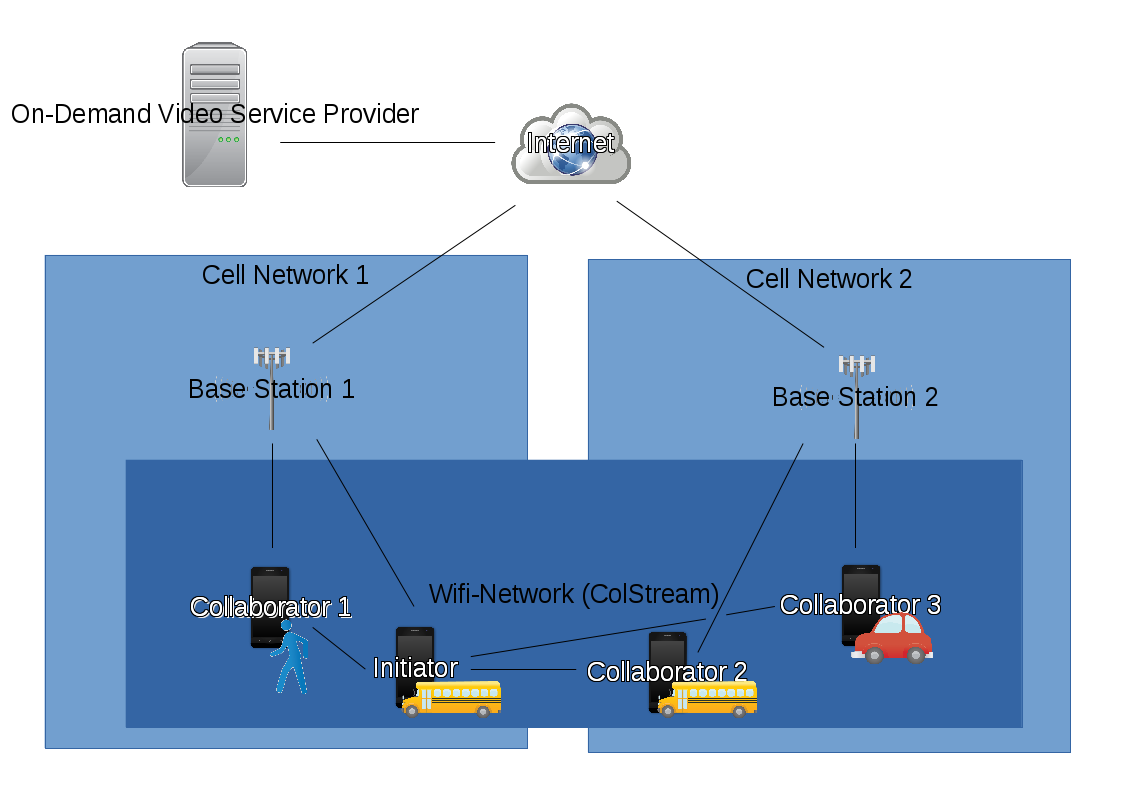
\includegraphics[scale=.6]{figures/Overview.png}
\caption{Overview of the idea of ColStream}
\label{ColStreamIdea}
\end{figure}
In \cite{ColStream} Zhong et al. describe a scenario of a person accessing a high-definition video stream through a mobile device over a 4G/LTE network. Figure \ref{ColStreamIdea} illustrates this scenario. The mobile network might experience interference or not be available at all times. To compensate for these limitations the mobile device connects over Wi-Fi to other mobile devices and negotiates with them the transmission of parts of the video stream over their 4G/LTE connection. As the location of the person is changing so is the level of experienced interference and the number and capabilities of devices surrounding it. ColStream promises to adopt to these changes and through negotiations to find the best available combilation of collaboration partners. The base for this negotiation process is provided by a virtual currency through which the video consuming participant can pay others who offer him their bandwidth.



\section{Related Work}\label{relWork}
There are a number of concepts and implementations that try to leverage cooperation to improve user experience when streaming or downloading information.
\subsection{Collaborative Download}
There are several Peer to Peer (P2P) networks that allow collaborative download. One famous example is the BitTorrent network which can be used to distribute large files like Operating System images with limited server capacity. Even though a streaming system with questionable legality was created based on it, these systems were designed to maximize the availability of a download, not its speed \cite{P2P}. When looking at streaming video to mobile devices, we assume the 3G/LTE connection to be the bottleneck. In this situation, the usage of such a P2P-system over this connection is of no advantage to us. While we could try to share information with our peers over Wi-Fi, we can not assume to have enough peers interested in the same information in range of our Wi-Fi connection.  
\subsubsection{CStream}
CStream \cite{CStream} appears to be a system very similar to ColStream, even in its naming, in which the C is short for collaborative. Both focus on the improvement of video streaming performance. However CStream does not focus on the mobile scenario. Instead it intends to apply this approach to a wider range of scenarios specifically including the combination of several wired connections.
\subsubsection{COMBINE}
COMBINE \cite{COMBINE} is a system designed to improve the download speed of files by using the 3G/LTE connection of other mobile devices, which can be reached over Wi-Fi. So it is very similar to CosStream, however it was designed without the realtime demands that appear when handling a video stream. Additionaly its current implementation only works on notebooks and PCs, not on smartphones or tablets. These two classes of devices still differ in many ways based on their processing power, the time they can work without recharging, the probability to find one of those devices turned on in your Wi-Fi range. We consider this to be problematic when evaluating the behaviour of this system on what we consider to be mobile devices.
\subsection{Incentive Systems}
One of the most important parts of ColStream is its incentive system, which is necessary to motivate users to offer their unused throughput to others. Unfortunately while the negotiation process for payment is discussed in depth, it is unclear if the system has any means to motivate the user to look for pazments to earn and to offer his available throughput to do so.In the following section we list a number of systems with a simmilar problem and their incentive approach.
\subsubsection{BitTorrent}
P2P networks face a similar problem. BitTorrent tries to evaluate the effort a user is providing based on his ratio of up- and downloads in relation to the resources available to him, specifically storage space and network access. Users can be punished for having a low ratio of uploads to downloads by restricting the download speed\cite{cohen2003incentives}.
\subsubsection{Webservices}
A number of webservices like reddit.com or duolingo.com allow the user to earn virtual points similar to the payments a user receives in ColStream. In the extreme case of reddit these points have no use besides showing others that a user has made valuable contributions. 


%%\label{chap:SomeStuff}

%% Note that the citations in this chapter use the journal and 
%% arXiv keys: I used the SLAC-SPIRES online BibTeX retriever 
%% to build my bibliography. There are also quite a few non-standard
%% macros, which come from my personal collection. You can have them
%% if you want, or I might get round to properly releasing them at 
%% some point myself.

%%\chapterquote{Laws were made to be broken.}%
%%{Christopher North, 1785--1854}%: Blackwood's Magazine May 1830

%%Symmetries, either intact or broken, have proved to be at the heart
%%of how matter interacts. The Standard Model of fundamental interactions
%%(SM) is composed of three independent continuous symmetry groups denoted 
%%$\SUgroup{3} \times \SUgroup{2} \times \Ugroup{1}$, representing the 
%%strong force, weak isospin and hypercharge 
%%respectively~\cite{Phys.Rev.Lett.19.1264, Phys.Rev.D2.1285,hep-ph/0410370}.

%%\section{Neutral meson mixing}
%%\label{sec:neutralmixing}
%%We can go a long way with an effective Hamiltonian approach in
%%canonical single-particle quantum mechanics. To do this we construct
%%a wavefunction from a combination of a generic neutral meson state 
%%$\ket{\Xzero}$ and its anti-state $\ket{\Xzerobar}$:
%%%
%%\begin{equation}
%%  \ket{\psi(t)} = a(t)\ket{\Xzero} + b(t)\ket{\Xzerobar}
%%\end{equation}
%
%%which is governed by a time-dependent matrix differential equation,
%
%%\begin{equation}
%%  \I \pdByd{}{t} \colvector{a \\ b}
%%  =  
%%  \underbrace{%
%%  \twomatrix{ M_{11}-\frac{\I}{2}\Gamma_{11}           
%%            & M_{12}-\frac{\I}{2}\Gamma_{12} }
%%            { M_{12}^\ast-\frac{\I}{2}\Gamma_{12}^\ast 
%%            & M_{22}-\frac{\I}{2}\Gamma_{22} }
%%  }_{\boldmatrix{H}}
%%  \colvector{a \\ b}
%%  .
%%\end{equation}
  \chapter{Technical Detail}

\section{Collaborative Downlaod}
ColStream assigns one of two roles to its users, initiators and collaborators. A user streaming a video is an initiator. Users offering their bandwidth to others are collaborators. The initiator creates a group of potential collaborators and assigns them chunks of the video stream data to download, based on their capabilities and price demands. The figures \ref{grpfrm1} and \ref{grpfrm2} illustrate the process of group formation, respectively the actual download of video information by role. 

\section{Group formation}

\begin{figure}[hbtp]
\centering
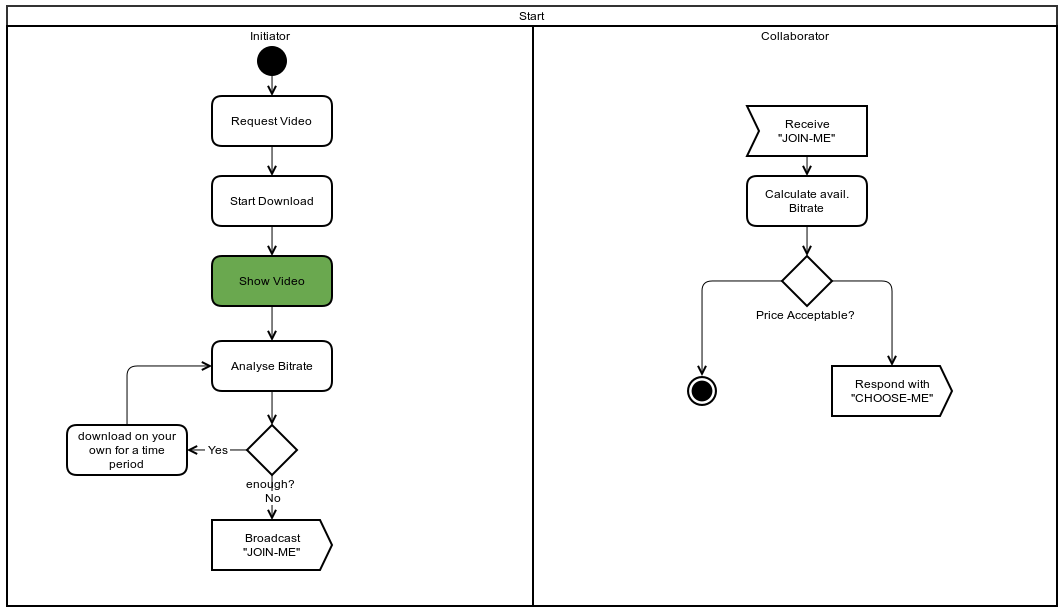
\includegraphics[scale=.6]{figures/Workflow_1.png}
\caption{Group formation}
\label{grpfrm1}
\end{figure}
% \label{groupformation1}


In the left half of figure \ref{grpfrm1} we see the behaviour of an initiator when he begins to stream a video. He starts by downloading and showing the video on its own. The initiator then analyses the bitrate at which he receives the video information. If this bitrate is enough to provide the user with an acceptable video quality, the initiator keeps streaming the video on its own and periodically rechecks the bitrate. Should at some point the bitrate be no longer acceptable, the initiator tries to form a group with collaborators. To find candidates for a group, the initiator broadcasts a "JOIN-ME" message. This message contains information on the amount of required bandwidth as well as how much the initiator is willing to pay for this bandwith. Potential collaborators in range of the initiator will receive the "JOIN-ME" request and process it as shown in the right half of figure \ref{grpfrm1}. Each collaborator first calculates the bitrate he could offer to the initiator based on the signal strength of the 4G/LTE network. He then compares the price offered by the initiator to his own current demand. Limited resources like battery capacity can drive the price up. Should the offered price be acceptable to the collaborator, he responds with a "CHOOSE-ME" message to indicate his consent to join the group.

\subsection{Bitrate estimation}
The collaborators estimate the bitrate they can offer to the initiator based on their signal strentgh. To be able to do this in a realistic way, collaborators periodically measure their signal and the corresponding bitrate. To compensate for fluctuations, historic information is factored into these measurements. The specific equations are 
\begin{itemize}
\item $signal=\alpha * signal_{new}+(1-\alpha)* signal_{old}$
\item $tp=\alpha * tp_{new}+(1-\alpha)* tp_{old}$
\end{itemize} with tp being throughput and \alpha an unspecified factor.

\section{Collaborative download}
The process of collaborative streaming within the group created in the previous section is shown in figure \ref{grpfrm2}.
Based on the "CHOOSE-ME" messages received by the initiator, a pool of possible participants in the streaming is created. The initiator then periodicly selects the best suited candidate to download a chunk of the video stream and assignes him this task by sending a request to do so. The size of the chunks is dynamically calculated to fit the throughput the candidates provide, using this equation:  \begin{itemize}
%{\frac{{MAX_CHUNK_SIZE * tp_{i}}{tp_{max}}}}equation  \begin{itemize}
%{\frac{{MAX_CHUNK_SIZE * tp_{i}}{tp_{max}}}}
\item $Chunk Size_{i}=\frac{MAX CHUNK SIZE * tp_{i}}{tp_{max}}$
\end{itemize}
Candidates are selected based on their price demand and offered bitrate. On receiving a download request, a collaborator downloads the assigned chunk of the stream and forwards it as a message to the initiator. When the initiator receives this message, he integrates the data into the video stream and displays it to the user.
The number of collaborators available to an initiator is expected to be changing over time. The collaborators send regular "I-AM-ALIVE" messages to the initiator to indicate that they are still available. They initiator will tolerate up to three missed messages in a row before dismissing the collaborator as not longer available.


%Workflow for the structure of collaboration
\begin{figure}[hbtp]
\centering
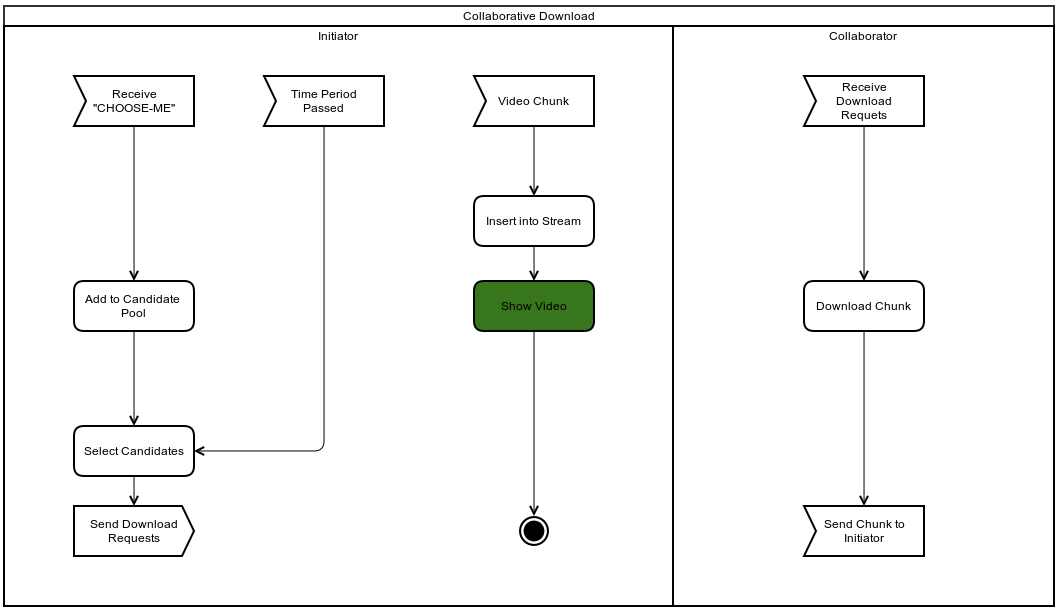
\includegraphics[scale=.6]{figures/Workflow_2.png}
\caption{Collaborative Download}
\label{grpfrm2}
\end{figure}


% \section{Working Algorighm}
\subsection{Problem handling}
The work is distributed between collaborators through assignment of chunks of the video. However once these chunks are assigned, a number of problems might appear that will make it impossible for the collaborator to complete the download on time. For example the user might experience interference which will drop his network throughput below the expected value. In this situation ColStream collaborators notify the initiator of the problem and forward the already downloaded information to him, so he has to reassign the remaining part only. Another problem is the loss of Wi-Fi connection to one of the collaborators. The initiator can notice this loss through missing "I-AM-ALIVE" messages or if the collaborator takes longer then expected to provide a chunk. If the collaborator does not respond to additional messages, the initiator will download this collaborators chunk on his own to compensate for the missing data.
  \chapter{Evaluation}\label{chap:ContCaptions}
To show the effectiveness of ColStream, Zhong et al. provide in \cite{ColStream} measurements they have collected in experiments. The scenarios for these experiments focus on its features, and one is a comparison with the COMBINE tool. The first is the increase of throughput by means of utilizing the network connection of several devices. The second is the adaptation to a changing number of available collaborators. We discuss these measurements in the following chapter. In the following four sections we discuss the experiments and results presented in \cite{ColStream} and point out aspects we consider problematic. The names of the respective sections follow the titles used in the paper.
\section{Experiment A: "basic tests"}
\subsection{Measurement Setup}
In these experiments ColStream runs on emulated android devices. One initiator and up to ten collaborators are emulated on a computer with an Intel Core i5-3210M processor and 6 GB of RAM. The paper claims that the throughput available to the individual emulated devices was fluctuated to make their behaviour more realistic, however the exact process of fluctuation is not disclosed. The initiators stream one of three videos from Youtube. These videos were randomly selected and differ in size. The time it takes for them to download the video was measured. The measurements were repeated with varying number of collaborators. 
\subsection{Results}
\begin{figure}[hbt]
\centering
\caption{Performance over number of collaborators \cite{ColStream}}
\label{performanceResults}
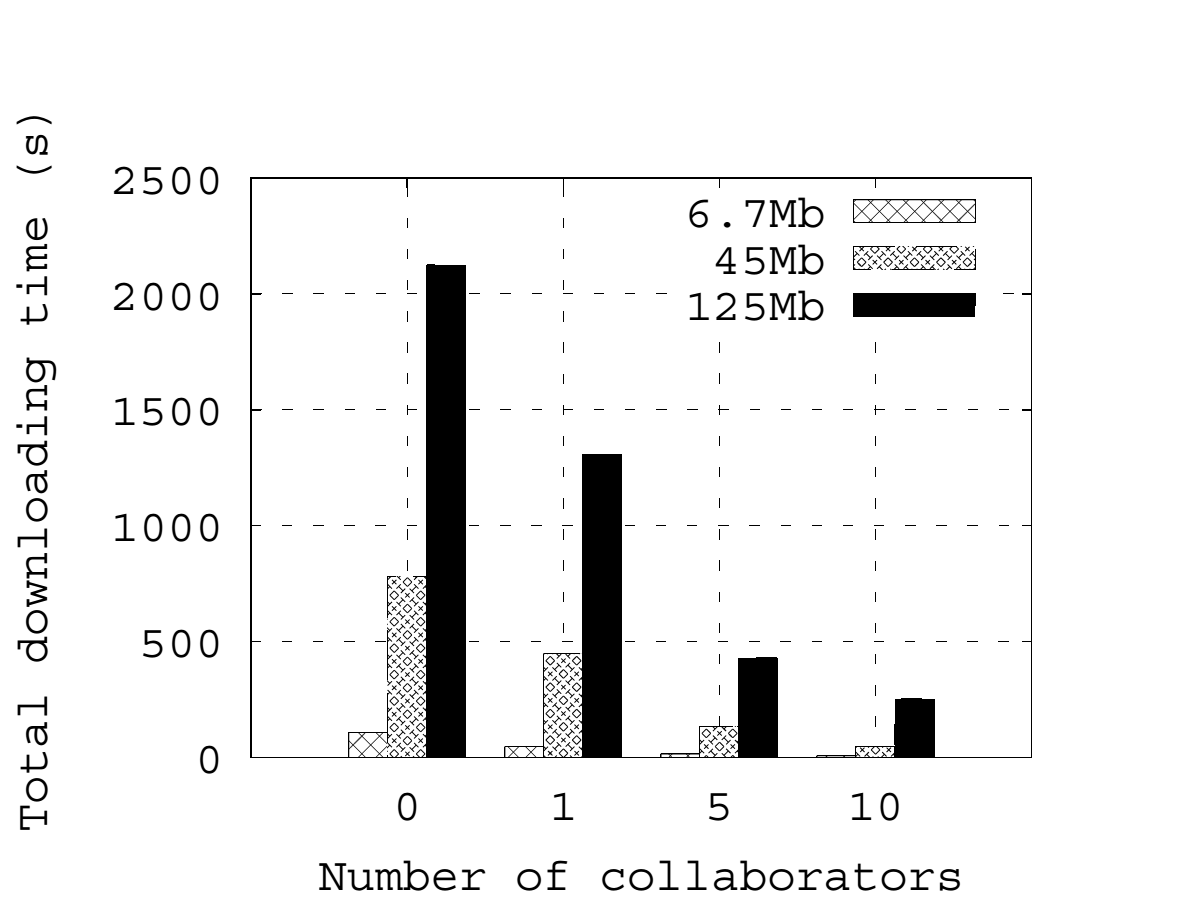
\includegraphics[scale=.5]{figures/Results.png}
\end{figure}
Figure \ref{performanceResults} shows the results as measured by Zhong et al. as a bar graph. The values are grouped by the number of collaborators used. Within each group, the time it took for this configuration to download each of the three videos is shown in seconds by the height of the corresponding bar. The size of the corresponding video for the bar is indicated by the pattern applied to it. This experiment shows that ColStream is able to reduce the time it takes to stream a video through employment of additional collaborators. In all three filesizes, the use of one collaborator already reduces the time by about a third. The improvement appears to increase with the size of the video to download.

\subsection{Criticism}
There are several aspects that raise the question if these results can be applied to a real world scenario. The paper provides very little information on the simulated network available to the emulated devices. One of the key motivations for the creation of ColStream is the compensation for fluctuation of throughput. Without knowing the strentgh of fluctuation applied to the throughput available to the streaming devices, these measurements can not be properly evaluated. Additionally these fluctuations seem to have been applied on the simulated 3G/LTE connection only, not on the Wi-Fi connection between the individual devices. The measurements were not repeated with different streaming platforms, files, networks or in any other variation. While these measurements do show as intended that ColStream could work, they do not show that it will work in any reliable way.


\section{Experiment B: "Dynamic adaptation"}
This experiment intends to show that ColStream is able to react to a changing group of collaborator. To do so, the streaming behaviour in reaction to collaborators joining and leaving the groups as well as price changes are demonstrated.
\subsection{Measurement Setup}
Unfortunately the measurement setup for this experiment is not explicitly stated. We assume the basic setup to be the same as in Experiment A, with emulated devices running on a notebook and experiencing a simulated fluctuation of network throughput. Three different situations are simulated. Number one is a new collaborator joining the group and demanding a lower price then the previously available collaborators. Number Two is a collaborator leaving the group. Number three is the loss of connection to one of collaborators.
\subsection{Results}
\begin{figure}[hbt]
\centering
\caption{Download ammunt over time by collaborator with user joining \cite{ColStream}}
\label{ColStreamJoin}
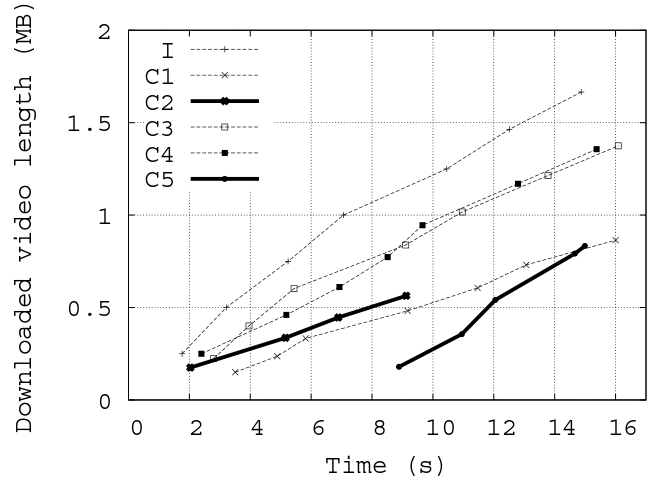
\includegraphics[scale=.5]{figures/ColStreamJoin.png}
\end{figure}
\begin{figure}[hbt]
\centering
\caption{Download amount over time by collaborator with user leaving \cite{ColStream}}
\label{ColStreamLeave}
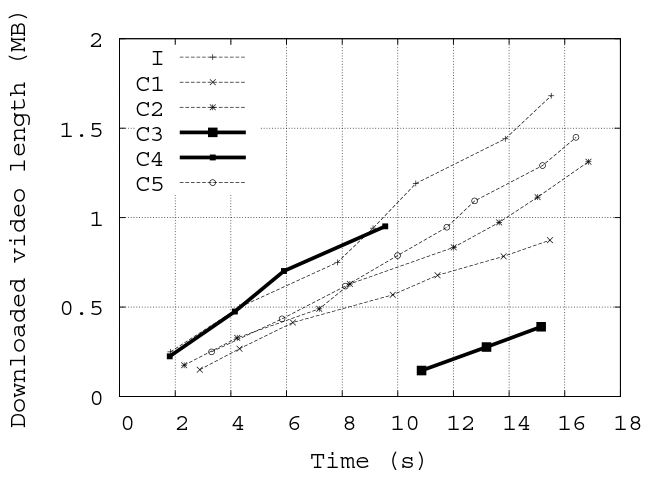
\includegraphics[scale=.5]{figures/ColStreamleave.png}
\end{figure}
\begin{figure}[hbt]
\centering
\caption{Download amount over time by collaborator with connection loss to user \cite{ColStream}}
\label{ColStreamReJoin}
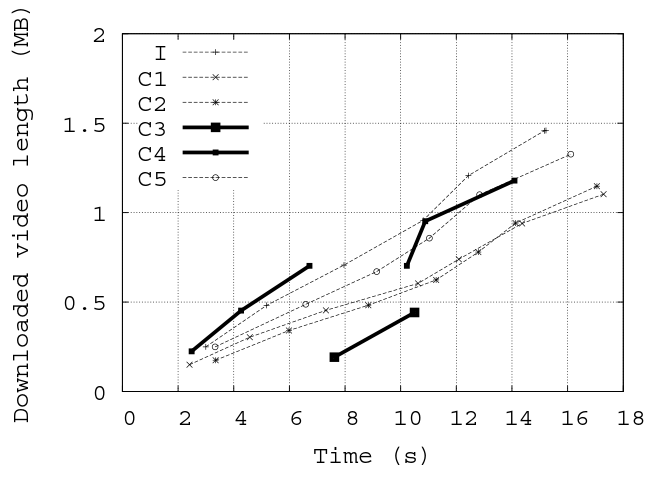
\includegraphics[scale=.5]{figures/ColStreamReJoin.png}
\end{figure}
The figures \ref{ColStreamJoin}, \ref{ColStreamLeave} and \ref{ColStreamReJoin} show the accumulated downloaded amount of data by collaborator over time. In all three figures the collaborators behave as expected. In figure \ref{ColStreamJoin} we see a new user (C5), demanding a lower price join after 9 seconds. As a result the user C2 is no longer assigned new parts to download. In figure \ref{ColStreamLeave} we see a user (C4) orderly leave and another user (C3) being selected as his replacement. Figure \ref{ColStreamReJoin} shows that colstream is able to handle a connection loss (at around 7 seconds) and its reestablishment (shortly after 10 seconds) to a collaborator(C4).
\subsection{Criticism}
While these measurements do suggest that ColStream could work as promised, unfortunately the influence of the collaborators leaving and joining on the quality of a videostream for the user is not made clear.

\section{Experiment C: "Performance tests: COMBINE agains ColStream"}
This experiment compares ColStream and COMBINE, which is also discussed in Section \ref{relWork} and intends to show that ColStream is better prepared to handle the specific challenges of distributed video streaming. To compensate for possible packet loss, chunks are assigned to multiple collaborators, to be sure to receive the information in time. This experiment looks at the amount of data that needs to be redownloaded by both systems, in reaction to random failures of collaborators.
\subsection{Measurement Setup}
Again very little is said to the setup of the experiment besides the use of five collaborators. While we can assume ColStream to be set up in a similar way as in the previous experiments, no such assumptions can be made about COMBINE.
\subsection{Results}
\begin{figure}[hbt]
\centering
\caption{Redownload handling by ColStream and COMBINE \cite{ColStream}}
\label{ColStreamCOMBINEComparisom}
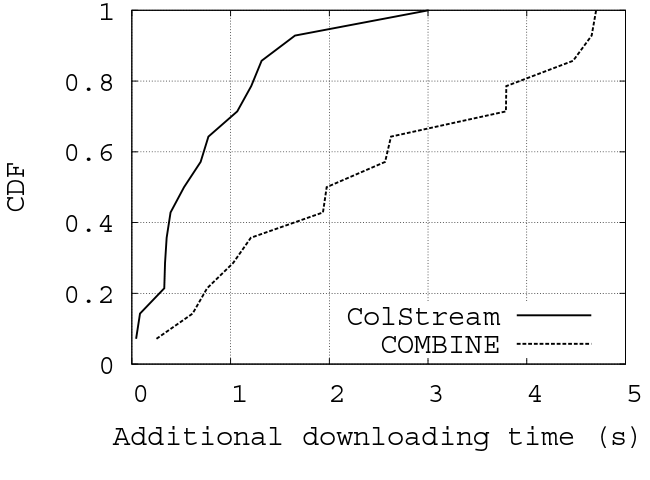
\includegraphics[scale=.5]{figures/ColStreamCOMBINE.png}
\end{figure}

Figure \ref{ColStreamCOMBINEComparisom} shows the performance of ColStream and COMBINE with growing additional downloading time on the x axis and their scores in a not exactly defined cumulative distribution function based benchmark on the y axis. ColStream is scoring higher at all measured values.
\subsection{Criticism}
Unfortunately it is in no way clear how reliable these benchmark tests are.

\section{Experiment D: "Feasibility study of the optimisation algorithm"}
This experiment measures the time it takes for ColStream to adjust to changing collaborator groups. This measurement allows to evaluate the amount of overhead generated by the group management and to decide if an initiator can adjust his peer selection fast enough to properly leverage changes in the group.
\subsection{Measurement Setup}
This experiment was executed on real devices with a range of hardware capabilities, specifically an HTC Desire C, Samsung Galaxy Nexus and a Samsung Note II. It was repeated for varying group sizes ranging from one to fifty participants. The time it took the initiator to adjust its peer selection is measured. Unfortunately it is not made clear if a video was streamed during this experiment.
\begin{figure}[hbt]
\centering
\caption{Group optimisation over group size \cite{ColStream}}
\label{groupAdjustment}
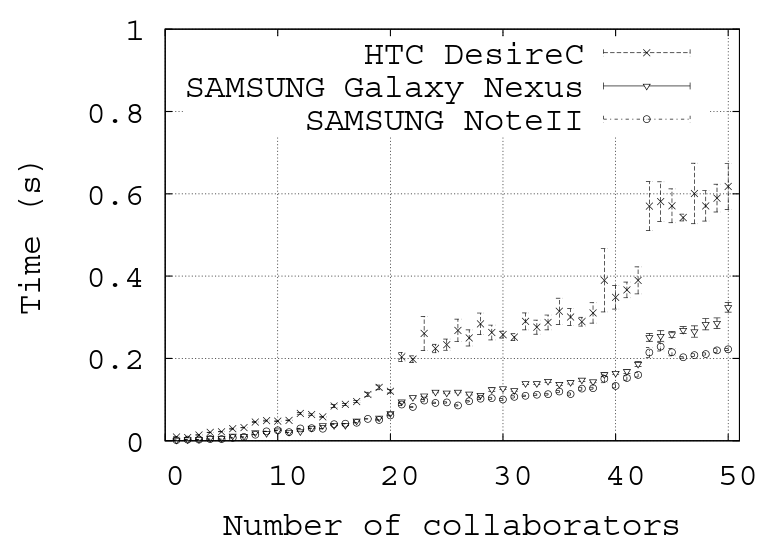
\includegraphics[scale=.5]{figures/ColStreamAdjustment.png}
\end{figure}
\subsection{Results}
Figure \ref{groupAdjustment} shows the group adjustment time on the y axis over group size on the x axis for the three devices. A clear trend of the adjustment time growing with the group size is visible. While the values for the two Samsung devices are close together, the Desire C takes longer to adjust.
This fits the much lower hardware characteristecs of the HTC device compared to the Galaxy Nexus. The Note II is the only device with a multi core processor. Since the peer selection algorithm is in no way prepared to make use of this, it is not surprizing that the measured values for the Galaxy Nexus and the Note II are close by. In all measurements, the values are low enough to assume that the group adjustment does not cause significant overhead.

\subsection{Criticism}
The previous section already looks at the hardware resources of the mobile devices to explain differences in measurements. However we think that the very similar values measured for the Samsung Note II and the Galaxy Nexus suggest that the measurements were executed without an actual video being streamed. We are not sure if these values would be of any significance to evaluate ColStream's ability to adjust to changes in collaborator groups.

\chapter{Criticism of the concept and implementation}
In the previous chapter we have already pointed out a number of concerns with the performance \cite{ColStream} promises for ColStream. However we think the concept of collaborative streaming in general and its implementation in particular raise a number of questions. As already discussed in Section \label{relWork}, a number of application rely on collaborative download. However the applications downloading a single file to all participants share an obvious common goal. This is not the case for ColStream and as the authors point out, they intend to compensate for this fact using the incentive system. However the concept of a price and compensation is only discussed on the subject of price negotiations. It is unclear how this virtual price would be paid and in what way the users are incentivized to aggregate payments. While it can be argued that this goes beyond the scope of ColStream as a proof of concept implementation and computer science in general, we consider the incentive system to be one of its most important elements. As the authors themselves argue, it sets ColStream aside other systems. As also stated in Section \ref{relWork}, one of the key features of BitTorrent is its upload to download rate based incentive concept. It would be interesting to make these values part of the incentive algorithm. The distribution of a collaborative download of a single file over a number of participants makes it unnecessary to hide the content of the downloaded file. This is no longer true if the collaborators purely assist in the download. This situation can pose a threat to the initiator as well as to the collaborators. The initiator obviously has to share information about the video stream he is requesting. By analyzing the price he is willing to offer and his demand for additional throughput, collaborators might deduct additional information about the initiator. The initator of course can make similar assumptions by identifieng the threshold acceptable price of collaborators. An additional problem for the collaborators is the fact that they are downloading content for another entity. If they don't evaluate the requested data, they might be used to download illegal or at least unlicenced content. If they do evaluate the requests or content, the initiator loses a lot of privacy.
A rather technical criticism is that a number of developer resources claim the simultaneous usage of Wi-Fi and and 3G/LTE on an Android device to be extremely limited if not impossible. While Zhong et al. state to have streamed video on real devices, the paper shows them only used for the evaluation of the video chunk selection and assignment algorithm. Unfortunately we were not able to find neither the sourcecode nor executable files of any kind that would allow us to recreate the measurements discussed here or extend them though our own experiments. So while the authors claim ColStream to be a good solution, there is no way for us to verify this claim. This appears to be a common problem in this area of research, since we ran into similar problems with other projects.
The result provided in \cite{ColStream} suggest that collaborative video streaming is at least technologically possible.

% http://forum.xda-developers.com/showpost.php?p=26408590&postcount=2

  %% To ignore a specific chapter while working on another,
  %% making the build faster, comment it out like this:
  %\input{chap4}
\end{mainmatter}

%% Produce the appendices
% \begin{appendices}
%   %% The "\appendix" call has already been made in the declaration
%% of the "appendices" environment (see thesis.tex).
\chapter{Pointless extras}
\label{app:Pointless}

\chapterquote[french]%
{Le savant n'\'etudie pas la nature parce que cela est utile; \\
\indent il l'\'etudie parce qu'il y prend plaisir, \\ 
\indent et il y prend plaisir parce qu'elle est belle.}%
{Henri Poincar\'e, 1854--1912}

Appendixes (or should that be ``appendices''?) make you look really clever, 'cos
it's like you had more clever stuff to say than could be fitted into the main
bit of your thesis. Yeah. So everyone should have at least three of them\dots

\section{Like, duh}
\label{sec:Duh}
Padding? What do you mean?

\section{$y = \alpha x^2$}
\label{sec:EqnTitle}
See, maths in titles automatically goes bold where it should (and check the 
table of contents: it \emph{isn't} bold there!) Check the source: nothing
needs to be specified to make this work. Thanks to Donald Arsenau for the
teeny hack that makes this work.

%% Big appendixes should be split off into separate files, just like chapters
%\input{app-myreallybigappendix}
% \end{appendices}

%% Produce the un-numbered back matter (e.g. colophon,
%% bibliography, tables of figures etc., index...)
\begin{backmatter}
  % \begin{colophon}
%   This thesis was made in \LaTeXe{} using the ``hepthesis'' class~\cite{hepthesis}.
% \end{colophon}

%% You're recommended to use the eprint-aware biblio styles which
%% can be obtained from e.g. www.arxiv.org. The file mythesis.bib
%% is derived from the source using the SPIRES Bibtex service.
\bibliographystyle{h-physrev}
\bibliography{mythesis}

%% I prefer to put these tables here rather than making the
%% front matter seemingly interminable. No-one cares, anyway!
\listoffigures
% \listoftables

%% If you have time and interest to generate a (decent) index,
%% then you've clearly spent more time on the write-up than the 
%% research ;-)
%\printindex
\end{backmatter}

%% Close
\end{document}